\documentclass[12pt]{iopart}
\newcommand{\gguide}{{\it Preparing graphics for IOP Publishing journals}}
%Uncomment next line if AMS fonts required
%\usepackage{iopams}  
\usepackage[utf8]{inputenc}
\usepackage[T1]{fontenc}
\usepackage{biblatex} %Imports biblatex package
\usepackage{lineno}
\usepackage{graphicx}
\linenumbers
\usepackage[normalem]{ulem}

\addbibresource{sample.bib}

\begin{document}

\title[cLACIr: Cognitive Load and Canine Intervention Recognition Dataset]{cLACIr: Cognitive Load and Canine Intervention Recognition Dataset}

\author{Walker S. Arce}
\address{University of Nebraska-Lincoln, Department of Electrical and Computer Engineering, Lincoln, 68588, United States}
\ead{wsarcera@gmail.com}
\vspace{10pt}

\author{Jeffrey R. Stevens}
\address{University of Nebraska-Lincoln, Department of Psychology, Lincoln, 68588, United States}
\ead{jeffrey.r.stevens@gmail.com}
\vspace{10pt}
\begin{indented}
\item[]September 2025
\end{indented}

\begin{abstract}
Emotionally intelligent machines require the ability to differentiate emotional responses from humans from any background.  Naturally, each human's emotional responses, whether it's physiological, facial, or any other modality, can be very unique to the individual.  While these specific responses are unique though, there are underlying trends and patterns that can be understood when using larger sample sizes.  The Cognitive Load and Canine Intervention Recognition (CLACIR) dataset consists of 140 participants whose physiological responses to cognitive load and intervention are recorded using an Empatica E4.  The dataset is split into two groups of participants which are roughly equivalent in size and separated temporally.  Physiological data consists of 3-axis accelerometry, electrodermal activity, and photoplethysmography recorded from the left wrist.  This dataset is useful as a baseline for assessing machine learning models as well as for pretraining or mixing with other datasets.
\end{abstract}

%
% Uncomment for keywords
%\vspace{2pc}
%\noindent{\it Keywords}: XXXXXX, YYYYYYYY, ZZZZZZZZZ
%
% Uncomment for Submitted to journal title message
%\submitto{\JPA}
%
% Uncomment if a separate title page is required
%\maketitle
% 
% For two-column output uncomment the next line and choose [10pt] rather than [12pt] in the \documentclass declaration
%\ioptwocol
%
\section*{Introduction}

Human emotion and affect are physiological and behavioral reactions to changes in our environment [cite]. Some affective states may be easy to label (e.g., anger) but others may be more difficult to pin down (e.g., stress, anxiety). What's more, individuals vary greatly in how they experience affective states, with some experiencing intense emotions and others experiencing more muted emotions. The field of affective computing develops machines and algorithms that can detect human affective states using measures of physiological responses such as heart rate, breathing rate, skin conductance, and muscle activation \cite{picard2000affective}. These physiological data are input into algorithms that attempt to classify the affective state experienced when the data were collected. [Need to give short explanation for why this is important. What does affective computing achieve?]

\sout{When applying machine learning to a vision-based task, ImageNet---a common dataset for pretraining vision models---contains 14 million images across twenty-thousand categories \cite{deng2009imagenet}.  The concept of pretraining utilizes the idea that there are underlying structures or patterns that are transferable to most, if not all, classification tasks.  In many cases, this is accomplished by training a machine learning algorithm on a very large structured, or unstructured, dataset so that the model can learn useful, generalizable features.}  

Accurately classifying human affective state requires large data sets due to the variability in emotions experienced within and between people. But the number of large-scale datasets for physiological signals is limited. Collecting physiological data can be difficult because participants must wear recording equipment either during their daily life or in a laboratory study \cite{gjoreski2020datasets, spathis2020learning, schmidt2018introducing, goodwin2019predicting, thayer2022effects, hosseini2022multimodal, poh2010wearable, ekiz2020can}.  The human body generates physiological signals through chemical and electrical interactions with various organs, which are largely involuntary and not easily controlled by an individual \cite{goodwin2019predicting}.  Consequently, targeted emotional states must either be induced in participants within a laboratory setting or annotated through surveys from naturalistic settings. Certain cognitive tasks can be used to reliably induce physiological states. For instance, researchers can put participants into a state of \textit{cognitive load}---where cognitive limits of processing information are strained---by engaging long-term memory, working memory, and attentional control [cite] \sout{\cite{thayer2022effects}}. Physiological measures show that cognitive load can cause stress-like responses in the autonomic nervous system, including changes in heart rate, heart rate variability, and galvanic skin response [Portnova et al. 2023; \url{https://doi.org/10.1007/s11055-023-01394-9}]. However, previous work has found ways to discriminate cognitive load from stress. Notably, Setz et al. 2010 found ... [Need to add in what we already know about detecting cognitive load from Setz et al 2010 \url{https://doi.org/10.1109/TITB.2009.2036164} and Markova et al. 2019 \url{https://doi.org/10.1109/BIA48344.2019.8967457}].
\sout{Currently, this limitation necessitates feature engineering, where humans decide which features to extract from a dataset to feed into a machine learning model \cite{picard2000affective, spathis2020learning, schmidt2018introducing, goodwin2019predicting, thayer2022effects}.  }




[Sorry, but this part below feels like justification for methods rather than an introduction to the study.]

\sout{Due to a lack of larger datasets, many studies utilize the leave one subject out (LOSO) approach, which excludes one participant as the testing set and uses the remaining as the training set \cite{schmidt2018introducing, farrahi2019evaluating}.  This has preference because it maximizes the amount of data used in training while also implementing an identity split, where a separate person, whom the model has never seen, is tested. It is possible that the excluded participant is the participant that the trained models perform the best on, which would be an unrealistic estimation of both the amount of variance between participants and the generalizability of selected features \cite{mac2002problem, li2006reduction}.  One method to remedy this is to balance the representation of each participant and each class and to perform multiple splits of the dataset based on these representations, rather than just each class \cite{li2006reduction}.  This method is called a stratified, group, k-fold split, which balances the class representation and the participant representation across k-folds \cite{pedregosa2011scikit}.  }

\sout{Additionally, collecting physiological datasets can be difficult because participants must either wear equipment during their daily life or participate for a short period using laboratory equipment \cite{gjoreski2020datasets, spathis2020learning, schmidt2018introducing, goodwin2019predicting, thayer2022effects, hosseini2022multimodal, poh2010wearable, ekiz2020can}.  The time-series physiological signals being measured are generated by the human body through chemical and electrical interactions with various organs, which are largely involuntary and not easily controlled by an individual \cite{goodwin2019predicting}.  Consequently, targeted emotional states must either be generated in participants within a laboratory setting or annotated through surveys from naturalistic settings by the participant.  Cognitive tasks can also be used to reliably generate physiological signal changes in participants, using tools such as the Deese-Roedinger-McDermott task to test long-term memory, the Necker cube pattern control to test attention control, the backwards digit span to test working memory, and the n-back to test working memory \cite{thayer2022effects}.  The labor required for these and other methods contributes to the low participant counts as well as to a low number of emotive states within the recorded data.  }

\begin{figure}[ht]
\centering
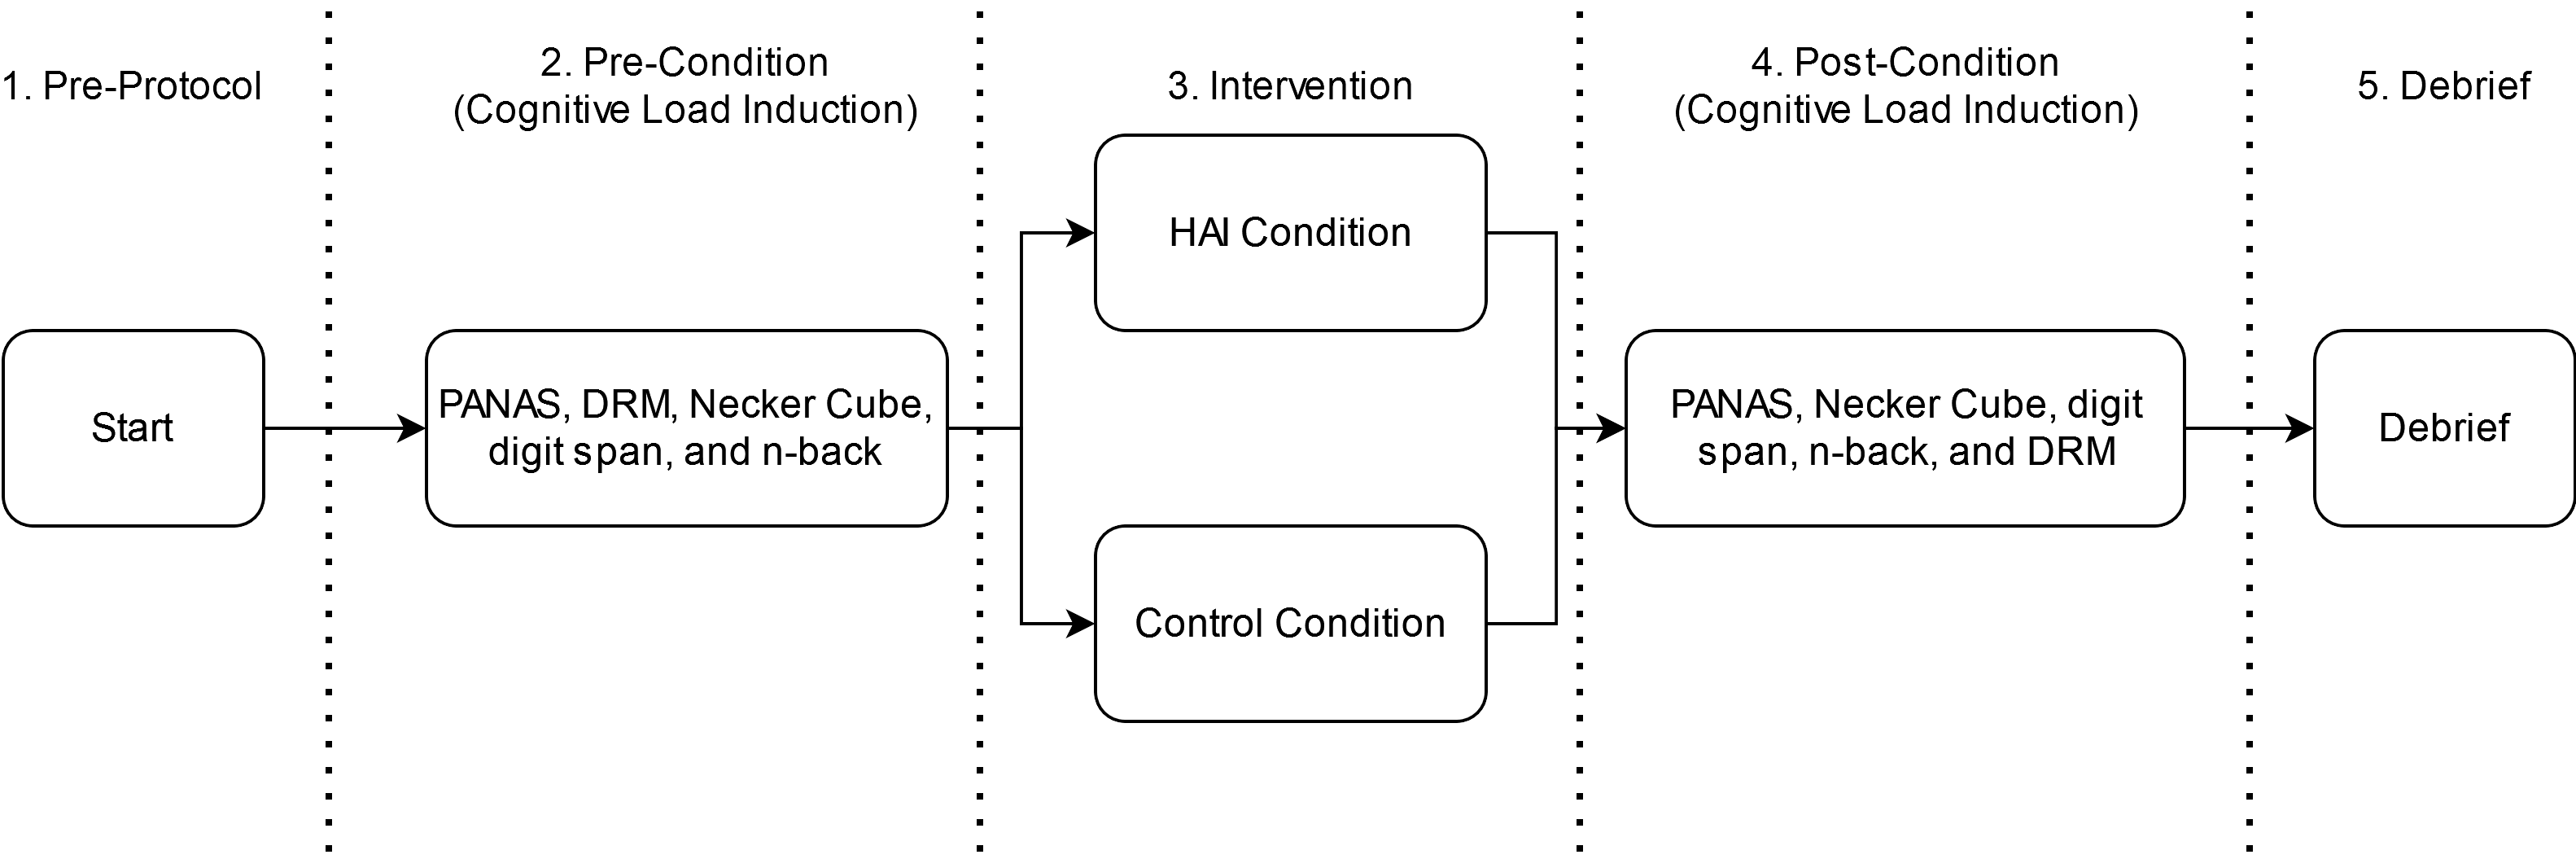
\includegraphics[width=\linewidth]{protocol.png}
\caption{The experimental protocol to induce cognitive load states and provide intervention from the same using a control and human animal interaction (HAI) conditions.}
\label{fig:protocol}
\end{figure}

Here we introduce the Cognitive Load and Canine Intervention Recognition (cLACIr) dataset, which provides multimodal physiological data from a variety of mental states including active cognitive load, control intervention, active intervention, and post-intervention cognitive load. The dataset comes from a study of how human-animal interactions influence mood, stress, anxiety, and cognition \cite{thayer2022effects}. The study tested 140 participants in three experimental phases: pre-condition, intervention, and post-condition (Figure \ref{fig:protocol}). The pre-condition phases tested participant long-term memory, attentional control, and working memory.  After completing these cognitive tasks, participants entered the intervention condition in which they either interacted with a dog (active intervention) or completed a repetitive task (control intervention). After the intervention, participants completed the same cognitive tasks. The \citename{thayer2022effects} paper analyzed the cognitive and mood data but not the physiological data collected during the study. Physiological data included 95.8 hours of data on blood volume pulse, electrodermal activity, temperature, and movement from 140 participants.


\sout{Due to the size of this dataset, large identity splits can be achieved, providing a fair method of comparing different machine learning architectures. } The aim of this study is to make available this large physiological data set, which can be used for affective computing. Moreover, we apply some preliminary machine learning analyses to investigate how the four physiological measures can be used to predict affective state. With cLACIr as a foundation, clinical applications can use machine learning for pilot studies in addition to traditional statistics \cite{phippsassessing}, more robust machine learning models can be incorporated into digital domains like virtual reality \cite{arce2021biosensor}, or can improve aggression detection approaches \cite{goodwin2019predicting, arce2023detecting}. [I think this sentence needs more context and/or expansion. Otherwise, it should be moved to the Discussion since it is more about the implications of this work than introducing what we did.]

[I think we need to end with the research questions that we pre-registered.]

\section*{Methods}

\subsection*{Original Data Collection}
This dataset was collected as a series of two experiments to investigate the effect of human animal interactions (HAIs) on affect and cognitive ability of the participants \cite{thayer2022effects}.  The first experiment was conducted from September to November 2018 and recruited 73 participants, 13 of which identified as male (17.8\%) and 60 identified as female (82.2\%), with a mean age of 19.2 (SD = 1.4) years old.  The second experiment was conducted from November 2018 to April 2019 and recruited 83 participants, 17 of which identified as male (20.5\%) and 66 identified as female (79.5\%), with a mean age of 19.9 (SD = 1.8) years old.  All participants were recruited from the University of Nebraska-Lincoln's psychology subject pool and did not have a physical or emotional aversion to dogs.  

To collect this data, an experimental protocol was designed that would induce a state of cognitive load on the participant, then apply an intervention condition, and then apply another cognitive load condition (Figure \ref{fig:protocol}).  The cognitive load induction has four separate cognitive tasks: Deese-Roedinger-McDermott (DRM) to test long term memory \cite{roediger1995creating, mcevoy1999connection}, the Necker cube pattern control to test attentional control \cite{orbach1963reversibility, cimprich1993development, sahlin2016influence}, the backwards digit span to test working memory \cite{berman2008cognitive}, and the n-back to test working memory \cite{rich2007effects, cohen1994activation}.  These assessments were presented and responses collected using PsychoPy version 1.90.2 \cite{peirce2019psychopy2} running on a computer's 16-inch monitor with only the participant and researcher present.  

After the cognitive load state was induced in the participant, they moved on to the intervention condition.  Each participant was pseudo randomly assigned to either a human animal interaction (HAI) condition or a control condition.  For the HAI condition, the participant interacted with the second author's dog, who was a 65-pound, neutered, male Catahoula leopard mix that was Canine Good Citizen certified prior to the study.  For the control condition, the participant was alone in the room and provided a sheet of paper with a full page of Latin text and instructed to circle every "e" and "f".  The participant was informed that the task would not be graded and there is no penalty for wrong answers.  The intervention condition was performed for three minutes in both cases.  After the intervention condition, the participant repeated the cognitive load induction activity.

To measure the participant's affect, the Positive and Negative Affect Schedule (PANAS)\cite{watson1988development} was administered before each cognitive load induction.  The second experiment also added measures of anxiety, including present and general feeling of anxiety with the State and Trait Anxiety Inventory (STAI) from \cite{spielberger1999measuring} and their present feelings of anxiety using the Anxiety Visual Analogue Scale (AVAS) from \cite{cella1986reliability}.  Due to the new measures, the cognitive load induction tasks were modified to perform the AVAS first, then STAI, and then PANAS.

\subsection*{Physiological Data Collection}
To measure the physiological responses of the participants, an Empatica E4 biosensor was affixed to their left wrist. This wrist-worn biosensor has been used to generate data in many studies \cite{goodwin2019predicting, schmidt2018introducing}, is regulatory compliant and validated \cite{poh2010wearable}, and is the top rated device for patient populations served by the behavioral analysis clinics \cite{taj2018review}.  This biosensor has four sensors: 64 Hz blood volume pulse (BVP) using photoplethysmography (PPG), 4 Hz electrodermal activity (EDA), 4 Hz infrared thermopile, and a 32 Hz 3-axis accelerometer measuring accelerations in its inertial frame of reference \cite{goodwin2019predicting}.  When transitioning between states of the protocol (start -> cognitive load induction -> intervention -> cognitive load induction -> debrief) researchers pressed the button on the biosensor to place a marker in the datastream.  This marker labels each data point with its associated protocol stage during post-processing. Figure \ref{fig:records} provides a schematic representation of the hierarchical structure of the dataset.


\begin{figure}[!htb]
	\centering
	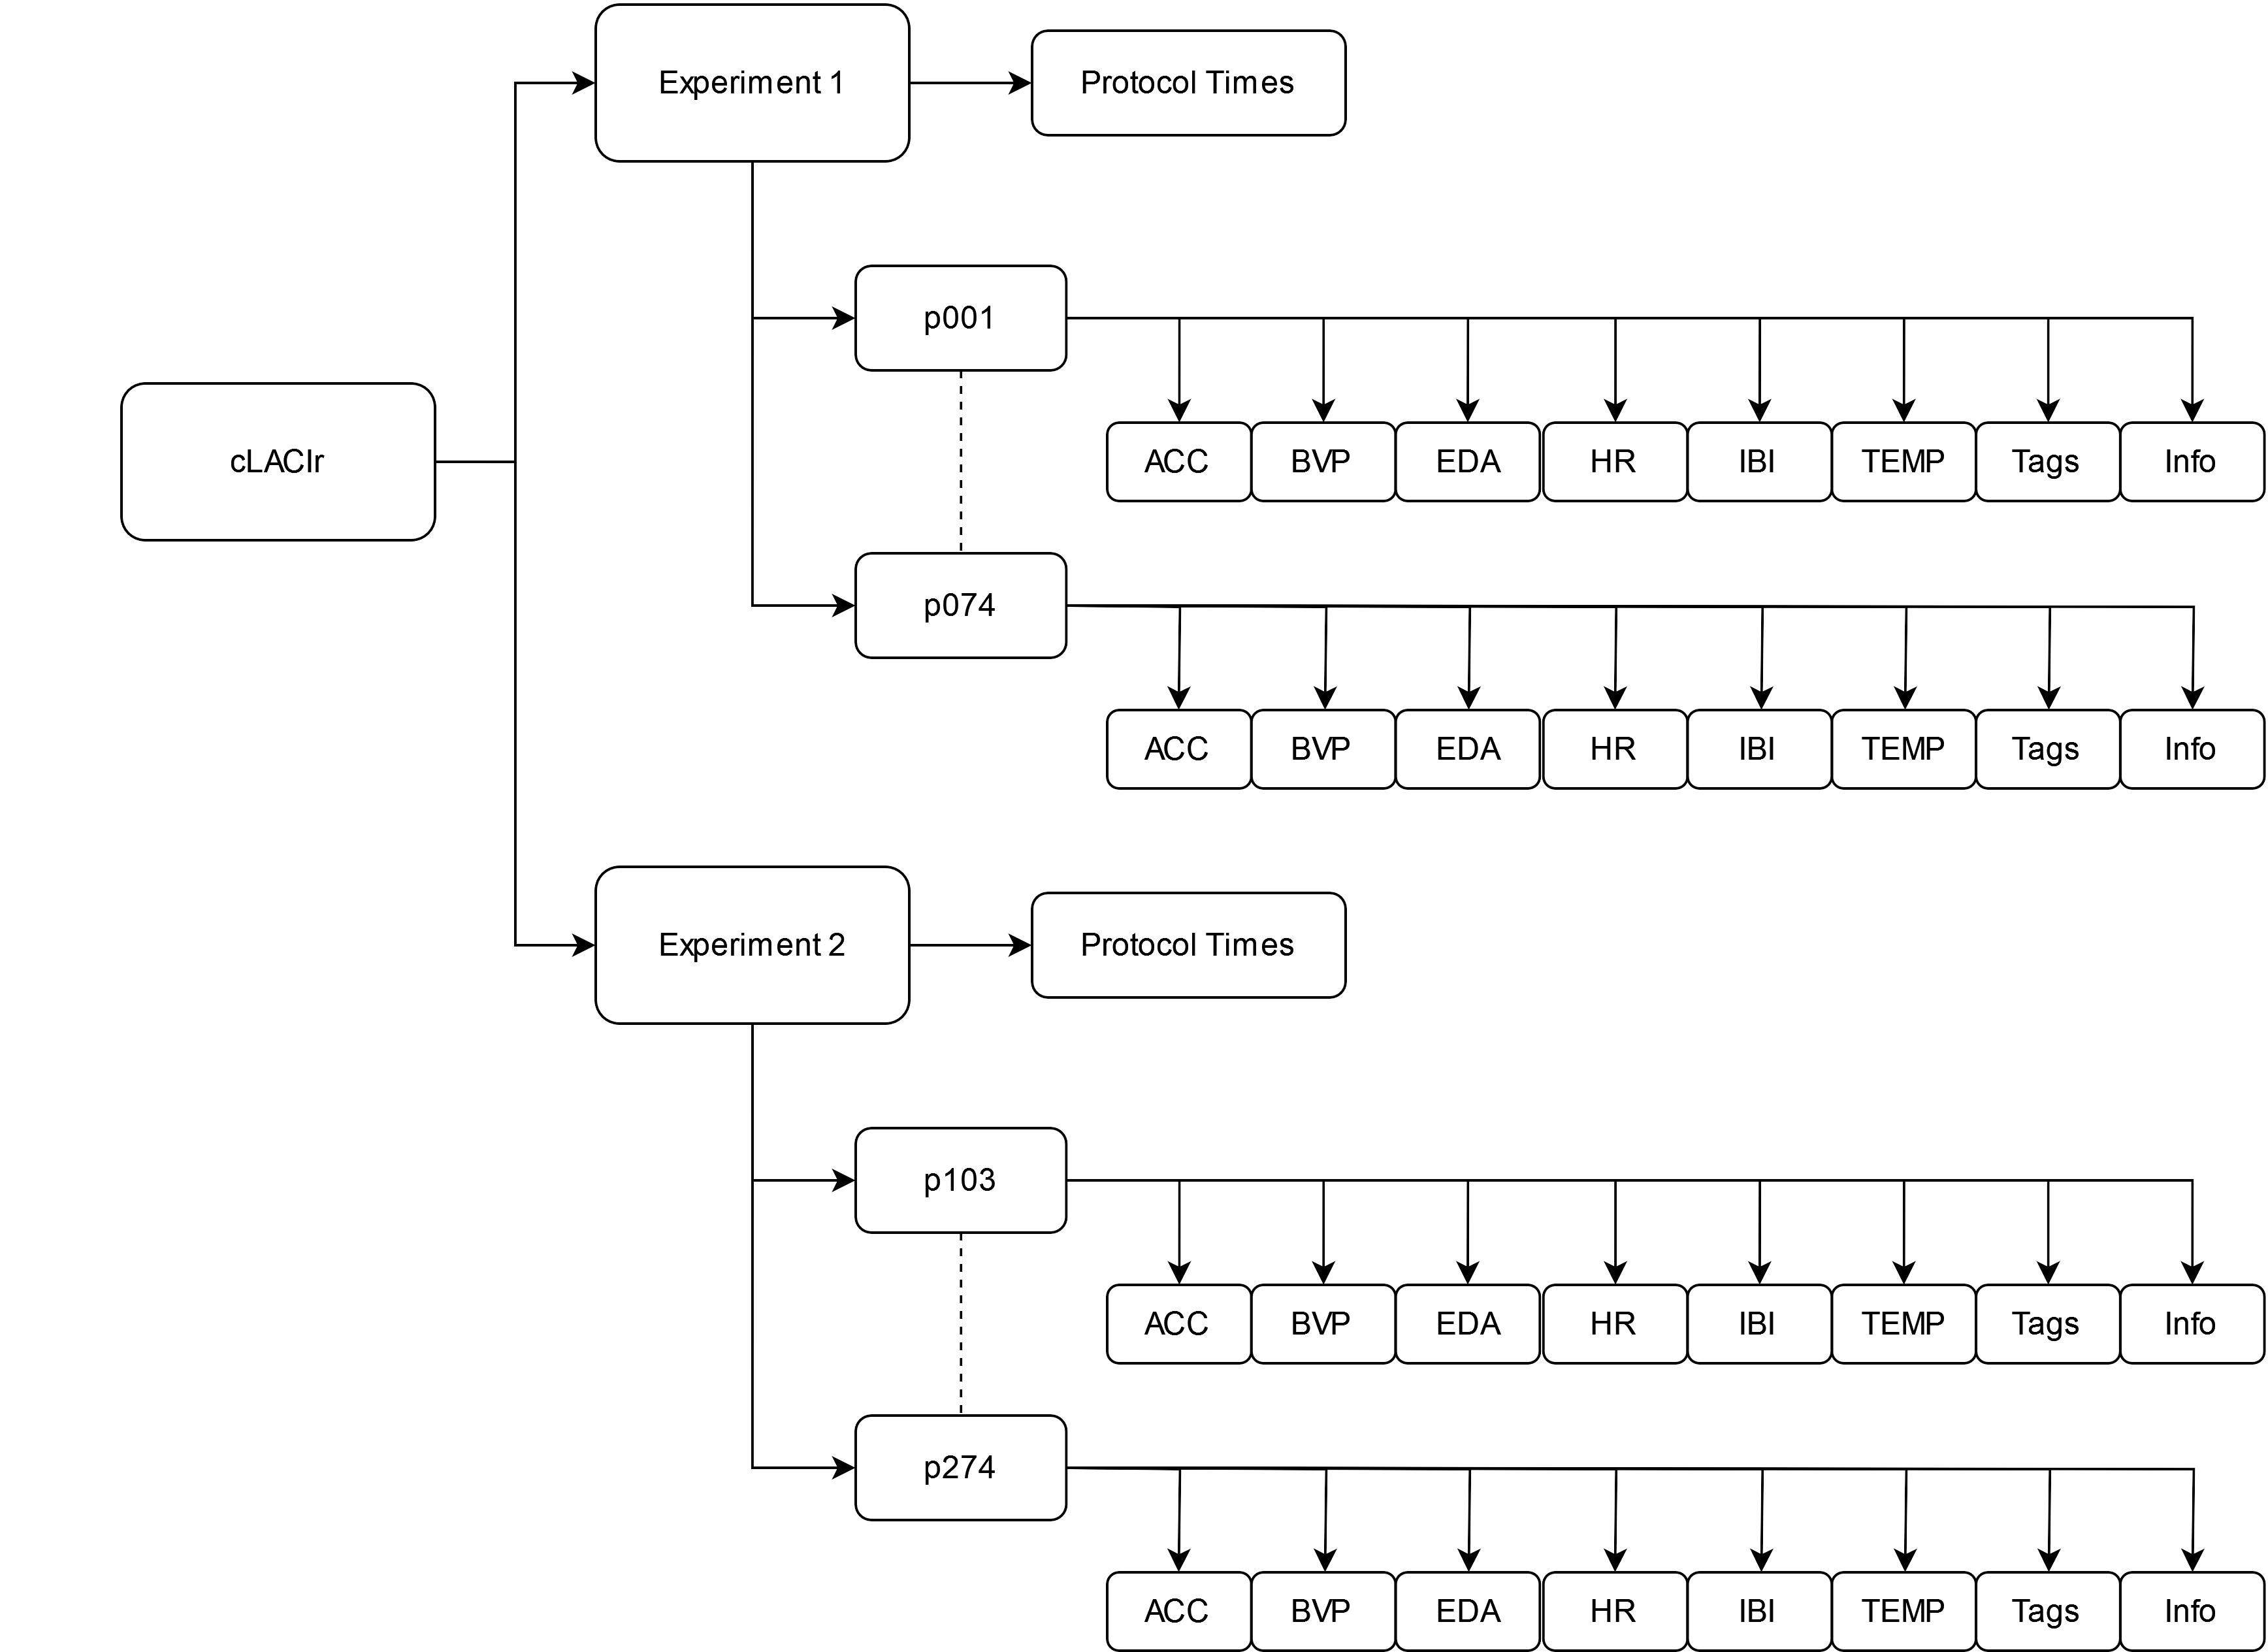
\includegraphics[width=\linewidth]{data records.png}
	\caption{The hierarchical structure of the cLACIr dataset. The dataset consists of two experiements with 73 and 83 participants respectively. For each participant, the dataset includes information on accelerometry (ACC), blood volume pulse (BVP), electrodermal activity (EDA), heart rate (HR), inter-heartbeat interval (IBI), body temperature (TEMP), and tags/markers signaling the experimental phase.}
	\label{fig:records}
\end{figure}


The E4 has multiple methods to compensate for common issues with in-situ physiological signal recording.  Measurement error in the PPG signal due to skin color and changing light intensity is compensated dynamically by the device \cite{goodwin2019predicting}.  Motion artifacts are removed from the captured signals and heart rate variability artifacts are removed as well \cite{goodwin2019predicting}.  Having this preprocessing be performed on the data before it is reported to the collection software reduces the burden on preprocessing for this experiment.  Due to this, minimal preprocessing is needed before training computational intelligence models.

Each physiological signal from the Empatica E4 encodes either physical movement of the participant (accelerometer) or their autonomic nervous system responses (PPG, EDA, thermophile).  By tracking the movement of the participant’s hand, specific movements that occur during emotional states can be assessed, which is the basis of physical activity recognition \cite{ravi2005activity}.  The separability of movements from different stimuli will likely be highly variable between participants and may be highly correlated to the level of reaction \cite{thang2012gait}.

Autonomic nervous system responses are highly correlated to internal emotional state \cite{kreibig2010autonomic} and are the basis of emotion recognition in ML systems \cite{healey2005detecting}.  The most common physiological signal used for this task is the EDA signal, which is collected by measuring the resistance between two contacts pressed against the participant’s skin \cite{society2012publication, arce2021biosensor}.  EDA data can be decomposed into three constituent signals: the skin conductance response (SCR), the skin conductance level (SCL), and noise \cite{greco2015cvxeda}.  The noise will be ignored.  The SCR is the fast-changing response to events, constituting a phasic component of the EDA signal, and can be used to approximate sympathetic nervous system activity \cite{society2012publication, benedek2010continuous}.  The SCL is a slower changing, tonic component of the EDA signal that acts as the baseline conductance of the skin.  These two components indicate how strongly an emotion was felt and can also be used to differentiate between emotional states, for instance, the SCL and SCR will go up when someone is feeling anxiety and only the SCL will go up if someone is feeling happiness \cite{kreibig2010autonomic}.  

Peripheral skin temperature is a common measure of stress and can be used to distinguish between emotional states \cite{collet1997autonomic, salazar2015mental, karthikeyan2012descriptive}.  Generally, the theory of blood flow constriction due to stress causing a decrease in skin temperature and blood flow dilation due to happiness causing an increase in skin temperature is used \cite{karthikeyan2012descriptive}.  But there are conflicting reports of skin temperature response to emotional states, where few report the temperature of the wrist or hand and instead focus on either monitoring facial temperature with a thermal camera \cite{salazar2015mental} or will place their temperature probe in an area that is free from thermal environmental disturbances, such as under the armpit \cite{karthikeyan2012descriptive}.  For studies that place the temperature probe on the hand \cite{collet1997autonomic}, a decrease in skin temperature is observed during happy states and an increase in skin temperature is observed for anger.  Considering the placement of the Empatica E4, the observations from the temperature probe on the hand will be considered.

Finally, PPG is an indirect method of measuring the cardiac cycle and can be compared with the electrocardiogram (ECG), which directly measures the electrical activity of the heart \cite{van2019heartpy}.  PPG is performed by measuring the change in skin coloration as blood travels through the capillaries of the skin, which is directly correlated to the blood being pumped by the heart (blood volume pulse---BVP).  From BVP, the Empatica system automatically calculates heart rate (HR) in beats per minute and the inter-beat interval of heartbeats (IBI).  In the case of someone feeling anxiety and happiness, their heart rate will go up \cite{kreibig2010autonomic}.  

Though the cognitive and affective data were reported in \cite{thayer2022effects}, the physiological data were not analyzed in the original study due to low sampling rate of the heart rate signal \cite{shaffer2017overview}.  The physiological data have been analyzed using machine learning in the first author's master's thesis \cite{arce2023unobtrusive}.  

\subsection*{Data Preprocessing}

To process the dataset, handcrafted features were extracted from overlapping 60-second windows of data.  These features consist of statistical information generated using the FLIRT toolbox \cite{foll2021flirt}.  The EDA signal is decomposed into its constituent signals (SCL, SCR, and noise) using cvxEDA \cite{greco2015cvxeda}. We kept the original signal, SCL, and SCR but discarded the noise component.  The other signals (PPG, accelerometry, and skin temperature) were processed in their original form using FLIRT.  The calculated statistics for each signal window were the mean, standard deviation, minimum, maximum, dynamic range, sum, energy, skewness, kurtosis, peak count, RMS, line integral, number of samples above and below mean, number of sign changes, 25\%-75\% interquartile range, 5\%-95\% interquartile range, 5-th percentile, and 95-th percentile.  Additionally, the entropy, perumutation entropy, and singular value decomposition entropy were calculated.  We calculated statistics for each signal broken into 5-second windows, which is a common approach \cite{schmidt2018introducing, phippsassessing}.  Each participant's data was tagged with their participant number, allowing the identity of the data to be tracked during training. 

We only analyzed data cognitive load, HAI intervention, or control intervention phases. We labeled data in this phase where the control intervention was considered neutral (label 0), cognitive load induction was considered stress (label 1), and HAI intervention was considered amusement (label 2), to align with \cite{schmidt2018introducing}'s labeling.  

For the binary task, the cognitive load class and HAI intervention are merged. To assess how induced cognitive load can be reduced through different intervention conditions, a second question that will be posed is whether the ML models can differentiate between post-condition that are preceded by the HAI intervention or control intervention.  The idea behind this question is that the level of cognitive load being experienced by the participant (and thereby recorded by the biosensor) is reduced in comparison to the control condition.  Both of these questions will be repeated for the condition where the accelerometry features are removed.  By including these features, we hypothesize that it is likely to be a naive discriminator for the models, where HAI can be detected by wrist movements caused by petting the dog. [I don't understand this paragraph. What is the binary task? What exactly is merged? What is the first question that we pose? How can we answer the second question if we don't differentially label the cognitive load phases (pre, post-HAI, post-control)? Maybe having the research questions at the end of the intro will help, but currently this paragraph is difficult to understand.]

\subsection*{Machine Learning Approaches}

The dataset will be benchmarked [How do you benchmark a dataset? I understand benchmarking an analysis but not a dataset.] using a standard selection of common machine learning models.  These models are Linear Discriminant Analysis (LDA), Decision Tree Classifier (DTC), Random Forest Classifier (RFC), and the K-Nearest Neighbors algorithm (KNP), all of which are implemented in SciKit-Learn \cite{pedregosa2011scikit}.  An LDA model uses a linear combination of features to separate two or more classes, where predictions are made using Bayes’ rule where the selected class maximizes the posterior probability \cite{hastie2009elements}.  These models are also closely related to analysis of variance (ANOVA), but the LDA uses continuous independent variables and categorical dependent variables \cite{wetcher2011analyzing}.  The DTC model uses simple decision rules, such as feature a is less than feature b infers class a, which makes predictions very explainable \cite{breiman1984nonlinear}.  The RFC is a meta-estimator that uses an ensemble of DTCs to predict classes based on the input data by taking a majority vote from the DTC ensemble \cite{breiman1999random}.  Finally, the MLP is a neural network that multiplies the input data by an input weight matrix, which is passed through an activation function and then finally multiplied by an output weight matrix, which produces several outputs proportional to the data classes \cite{hinton1990connectionist}.  These models are trained by adjusting the weight matrices using various backpropagation algorithms, such as the Adam optimizer that moves the operating point of the model using first- and second-order moments \cite{kingma2014adam}.

To train the machine learning models, a stratified group 10-fold approach was used \cite{pedregosa2011scikit}.  Using the identity labels, dataset features, and dataset labels, 10 splits of the data were generated, where each split contains a different group of identities and the number of samples from each class was as balanced as possible.  By doing this, not only will the test set contain unique identities from the train set, a requirement for generalization performance, but the choice of identity for testing can also be evaluated.  Doing this, a mean and standard deviation for each evaluation metric was generated.  If there are ideal and non-ideal choices for test participant, then this will be observed as a high standard deviation in the final metrics.  Finally, the PANAS results were used to filter out participants in the dataset by thresholding the difference between pre- and post-condition PANAS scores. The PANAS threshold represents [fill this in]. By varying this from -1 to 1, we can filter out participants who had an increasingly positive reaction to the data collection and see if the physiological data reflects this.

\subsection*{Figures of Merit}

While the training of ML models can be simplified to a few function calls using highly abstracted software libraries, the methods to compare trained models in a fair way is still an active question.  The most common method of comparison is accuracy, or more properly, top-1 accuracy.  This metric quantifies how often the highest probability class is the target class.  There is also top-k accuracy, which looks at an increasing number of output probabilities and, if the target class is in that list of probabilities, then it counts as correct [cite Liu, 2014].  For binary classification, there is only top-1 accuracy.  

The next most common metrics are recall- and precision-based metrics.  Recall as a metric quantifies how often the model correctly chooses a class versus the number of times that it should have chosen that class, while precision quantifies how often a class is chosen correctly versus all the times that class is chosen [cite Davis, 2006; Liu, 2014].  These two metrics can be combined to create derivative metrics, such as the F1 score, which is the harmonic mean of precision and recall [cite Liu, 2014] and can give insight into how well a model balances those two metrics.  At this level, these mentioned metrics are common across all ML analyses.  

Computer vision has utilized many robust metrics using receiver operator characteristic (ROC) curves to quantify the diagnostic ability of a binary classifier at varying threshold levels on the probability outputs [cite Davis, 2006; Fawcett, 2006; Liu, 2014].  For these curves, the true positive rate (TPR) is plotted on the y-axis and the false positive rate (FPR) is plotted on the x-axis for all values of the threshold from 0 to 1.  An optimal relationship between TPR and FPR occurs when the TPR is very high and the FPR is very low, meaning that the curve approaches the upper left corner of the plot.  The area under the curve (AUC) of the ROC curve is a way of capturing the curve in a single number, where the closer it is to one, the closer the ROC curve is to the upper left of the plot area.  Setting thresholds on the FPR can be useful for establishing a confidence level in the performance of a model.  If the FPR is set to 1\%, then a corresponding TPR of 95\% would indicate that for every 1 false positive (FP) prediction, 95 true positive (TP) predictions would be accomplished on average.  This is commonly extended to two or three thresholds, namely: 1\%, 5\%, and 10\%.  Equally important to mention is the equal error rate (EER), which is the ratio of the FPR to the false negative rate (FNR) by drawing a line from the top left corner of the ROC curve to the bottom right corner and finding the intersecting values [cite Jothilakshmi, 2016].  In this case, a lower value indicates that the classifier is performing better, and this metric is important when the risk of false positive or false negative identification is equally harmful.

While ROC metrics such as AUROC are used in affective computing research, it is not widespread and isn’t accompanied by other ROC metrics, such as TPR @ x\% FPR, which would provide heightened insight into the confidence of a classifier.  Other metrics are being discussed for affective computing, namely the area under the precision recall curve (AUPRC) and Cohen’s kappa coefficient \cite{d2018affective}.  AUPRC is constructed similarly to the AUROC, but precision is plotted on the y-axis and recall is plotted on the x-axis for all values of the threshold, when both metrics are high then the curve will increase towards the upper right corner of the plot area.  The larger the area under the curve, the greater the precision and recall at all thresholds.  This metric is also called average precision (AP) and in multi-class problems, the mean AP (mAP) is the average AUPRC across all classes.  Cohen’s kappa coefficient quantifies the inter-rater reliability, which is the degree of agreement between independent observers of the same phenomena, which can be considered a more robust accuracy measure because it takes the probability of random chance agreements into account [cite Cohen, 1960].  The concern of not using descriptive metrics is related to the way that AC tasks are constructed.  In most cases, the classification task of emotion vs. neutral has a data distribution that leans towards neutral [cite Schmidt et al. 2018; D’Mello, 2018].  Consequently, a model trained on this imbalanced data, i.e., 80\% neutral / 20\% emotion, then predicting zero (neutral) for every sample will generate a top-1 accuracy score of 80\% automatically [cite D’Mello, 2018].  Increasing in popularity, balanced accuracy seeks to improve top-1 accuracy by using the TPR plus the true negative rate (TNR) divided by two, which accounts for some of the class imbalance problems.

\subsection*{Pre-registration and Data Availability}
The analyses for this study were pre-registered at [URL]. Data are available at [URL].


\section*{Results}
\subsection*{HAI vs. Control Intervention Classification}

The first classification test of the dataset differentiated between the HAI condition and the control condition during the intervention stage of the data collection (Figure \ref{fig:intalldata}).  

\begin{figure}[!htb]
	\centering
	
\includegraphics[width=\linewidth]{Int All Data.png}
	\caption{The effect of using various thresholds on the PANAS score to exclude participants from dataset and training to differentiate between intervention conditions using data from intervention stage. PANAS threshold represents [fill this in]. Panels represent different measures of accuracy, including balanced accuracy, Cohen's kappa coefficient, area under the precision recall curve (AUPRC), and true positive rate at 10\% of false positive rate (TPR @ 10\% FPR). Individual lines represent mean$\pm$?? [what measure of error is this?] performance for decision tree classifier (DTC), k-nearest neighbors (KNN), linear discriminant analysis (LDA), and random forest classifier (RFC). For balanced accuracy, the black line represents the baseline value, which is the ratio of one class over another.}
	\label{fig:intalldata}
\end{figure}

With the full dataset (PANAS threshold of -1), there are clear improvements that can be achieved by selecting different models.  The RFC and LDA perform the best of the four, with balanced accuracy staying above 80\% during the ablation study. [What is an ablation study? This isn't mentioned before.] That is, using all of the physiological data, RFC and LDA can accurately classify the label as the HAI or control condition more than 80\% of the time. As the data gets restricted to [I don't remember exactly what PANAS threshold is. Fill in answer here], the accuracy is fairly constant with a slight bump to the balanced accuracy results when the PANAS threshold between 0.7-0.8. This indicates that removing participants who had a more negative reaction to the study [what does this mean?] improves the ability to differentiate between classes.  This contrasts with the other metrics, where AUPRC continues to drop as the PANAS threshold increases.  The Kappa test shows some loss in agreement between raters, but the TPR @ 10\% FPR shows a similar trend to the balanced accuracy, where it stays solid until the PANAS threshold is sufficiently high and it gets a boost.  The models all show similar comparisons to one another across metrics (no model outperforms another in one metric that it underperforms in another), which is not entirely unexpected.  Interestingly, the DTC model has a horrible TPR @ 10\% FPR, which steadily increases until as the PANAS threshold is tuned.

\subsection*{HAI vs. Control Postcondition Classification} 

The second classification test of the dataset differentiated between HAI and control conditions during the postcondition stage of the data collection (Figure \ref{fig:apalldata}).

\begin{figure}[!htb]
	\centering
	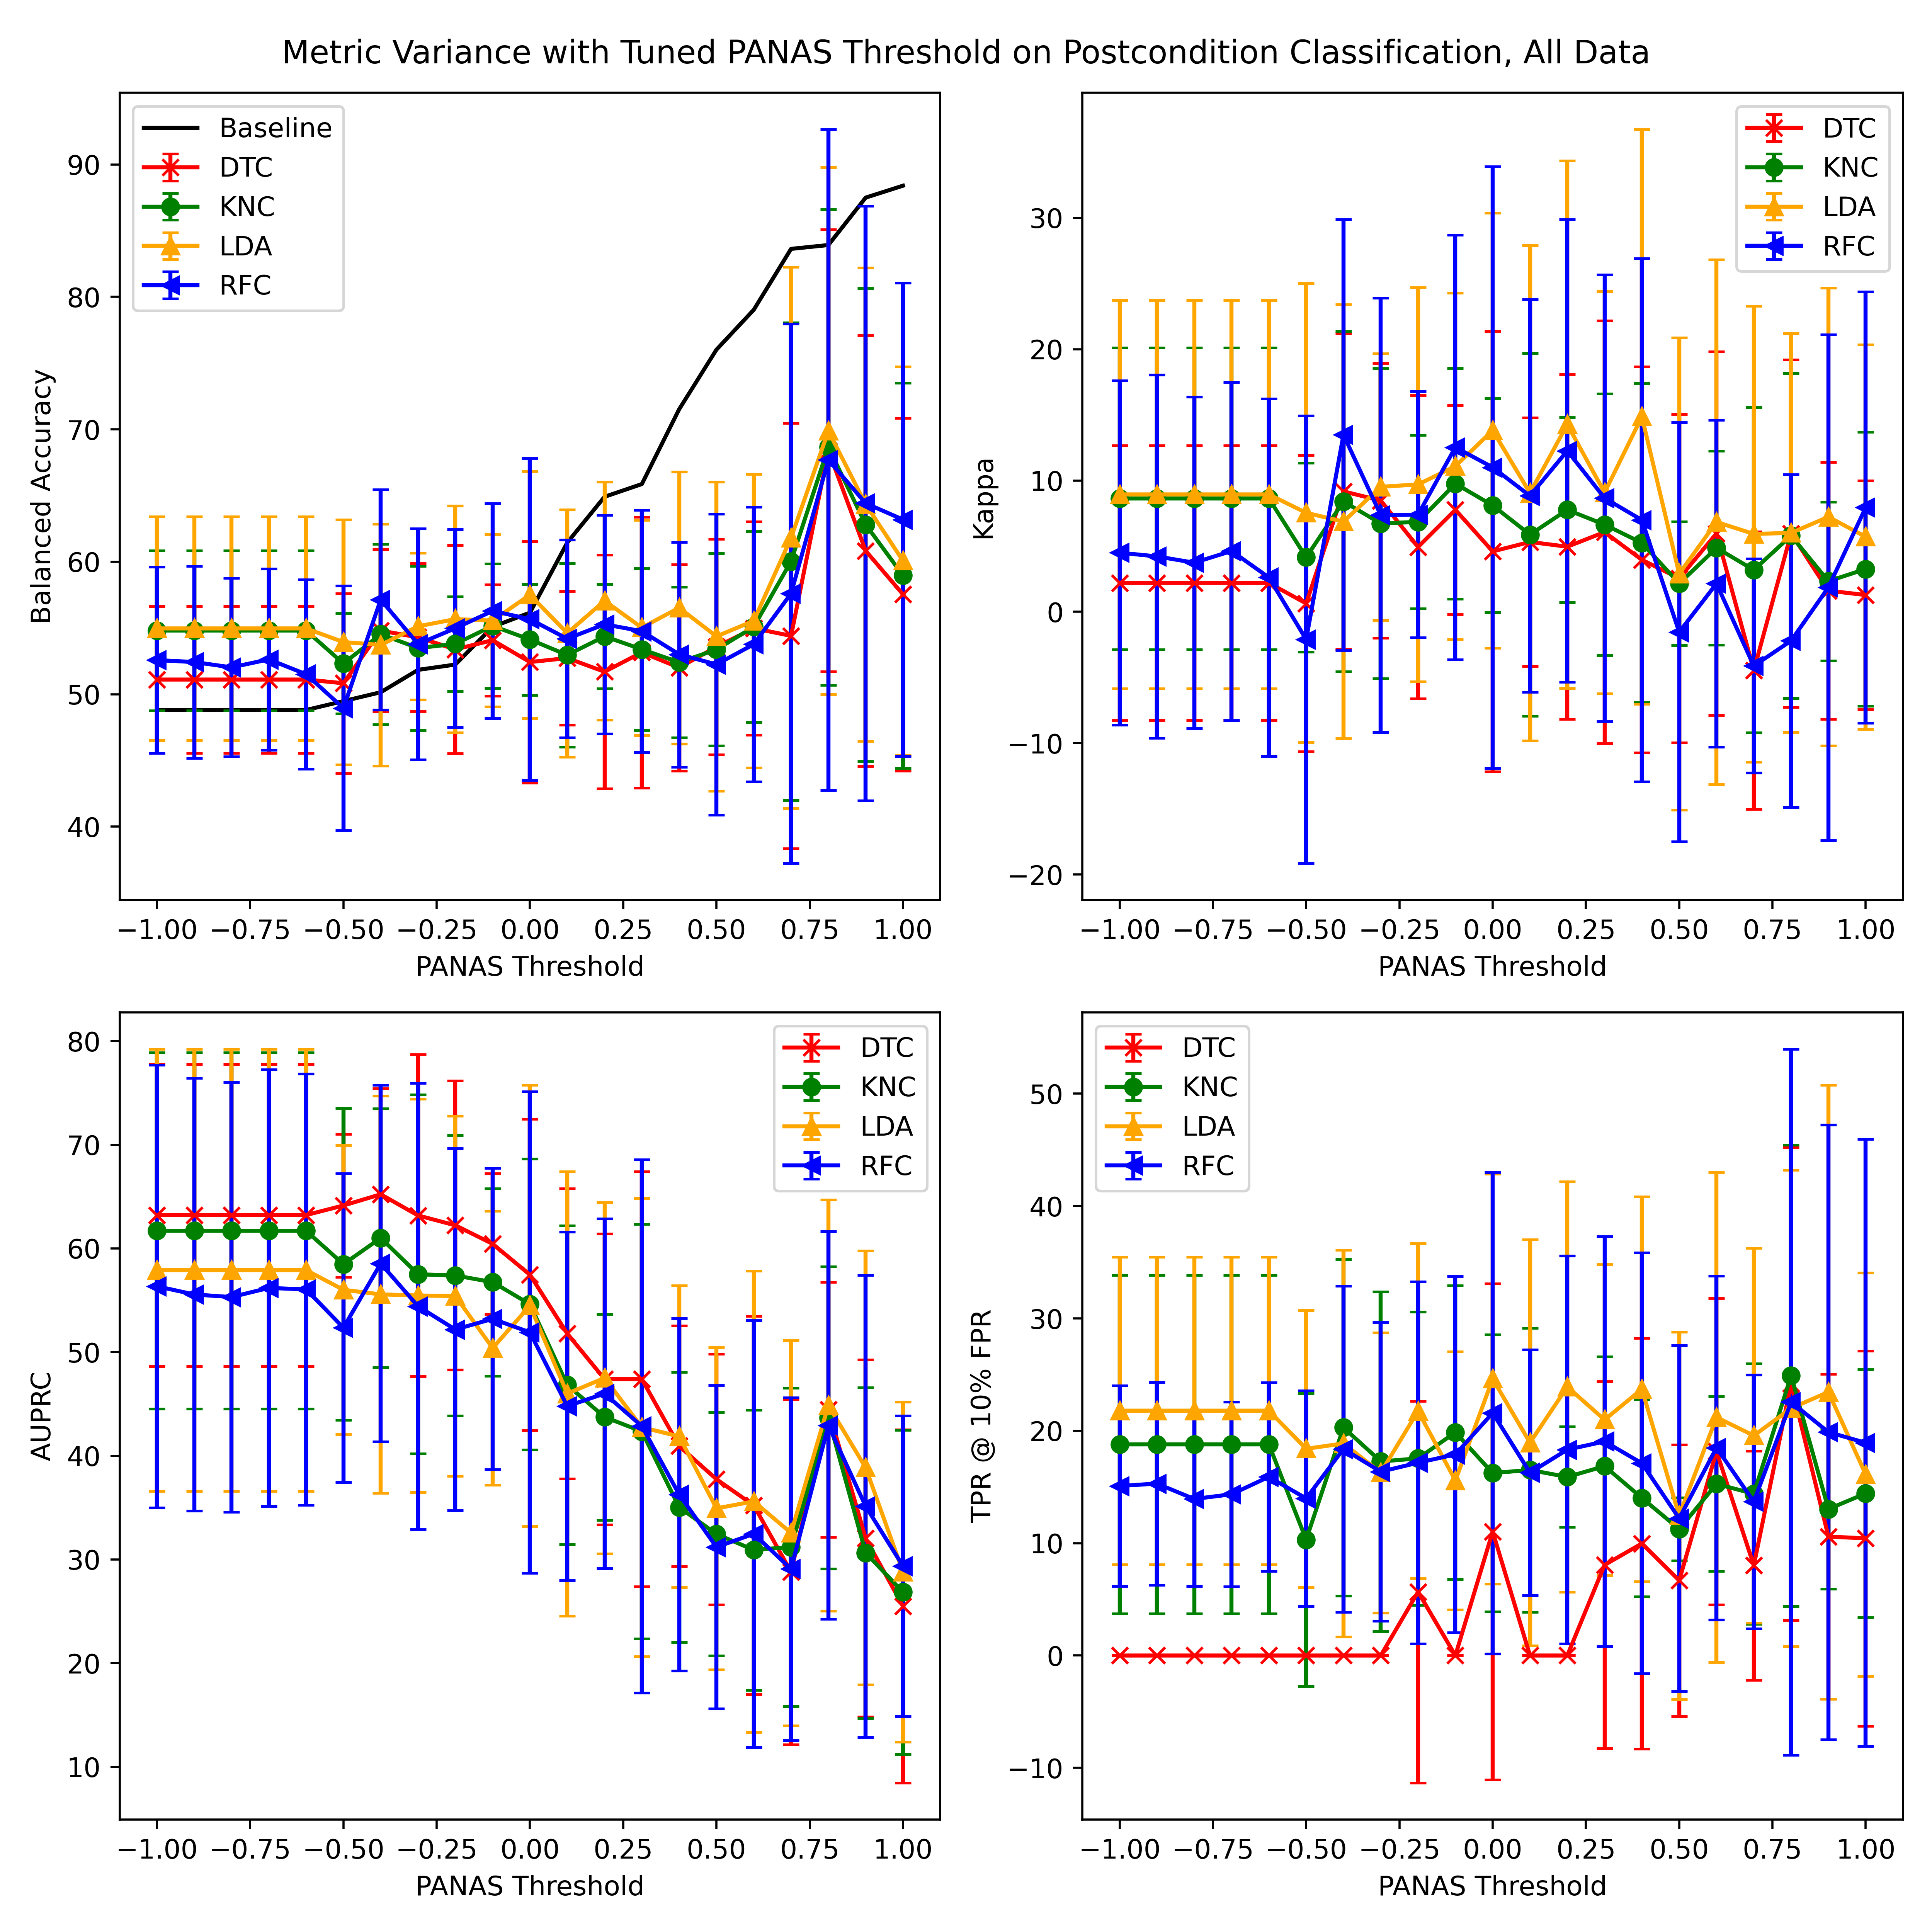
\includegraphics[width=\linewidth]{AP All Data.png}
	\caption{The effect of using various thresholds on the PANAS score to exclude participants from dataset and training to differentiate between intervention conditions using data from postcondition stage.  PANAS threshold represents [fill this in]. Panels represent different measures of accuracy, including balanced accuracy, Cohen's kappa coefficient, area under the precision recall curve (AUPRC), and true positive rate at 10\% of false positive rate (TPR @ 10\% FPR). Individual lines represent mean$\pm$?? [what measure of error is this?] performance for decision tree classifier (DTC), k-nearest neighbors (KNN), linear discriminant analysis (LDA), and random forest classifier (RFC). For balanced accuracy, the black line represents the baseline value, which is the ratio of one class over another. }
	\label{fig:apalldata}
\end{figure}

This classification task is much more difficult, because participants were no longer in their intervention stage, so if they are in an excited state, then they are relaxing from it.  This is reflected in the data, where the models perform similarly and balanced accuracy for this task hovers slightly above the baseline performance.  Even as the PANAS threshold is tuned, poor performance continues until around a PANAS threshold of 0.75, where a spike occurs.  It doesn't reach the baseline value, but it increases to nearly 70\% with all models.  The same trends occurred for the other metrics.    


[Does this cover all of the analyses that we pre-registered?]

%\subsection*{Dataset Mixing}
%When mixing cLACIr with other datasets, WESAD and CASE, and evaluating using the methods in this paper, the standard deviation always drops significantly in comparison to either dataset.  In physiological datasets that have actual test sets, you will see wide ranges on the standard deviation, this implies that participant selection matters.  This is most prevalent on small datasets, where the training dataset is prioritized for size against the test dataset, leading to a significant imbalance.  cLACIr breaks this trend through size, where the test set comprises over a dozen individuals and has a figure of merit performance that outperforms all other datasets while maintaining low standard deviation between folds.
%
%things to do:
%1. Perform evaluation on all folds so I get the mean and SD of those
%2. Rerun the cLACIr baseline tasks for self performance
%3. Separate test dataset performance by dataset, so mean and SD can be assessed for test participants in CASE vs. cLACIr, for example


\section*{Discussion}

Our dataset performs at the same level as other similar datasets.  WESAD, with 15 participants, achieves upper 70\% and lower 80\% top-1 accuracy results across the board, the DT model performing the worst \cite{schmidt2018introducing}.  \cite{gjoreski2020datasets} had a wider variety of top-1 accuracy values, but achieved a peak value of 82.3\% using their Snake dataset and 68.2\% using their cognitive load dataset, each with 23 participants.  These two examples shows that cLACIr either outperforms or is on par with other similar datasets.  Through the sheer number of participants, our models show generalization in our task that is not able to be explored in other datasets due to limited participant count.  

It is possible that there is a "cooldown" factor after a participant experiences the HAI condition, such that breaking up the postcondition classification by time bins would improve the accuracy.  It is also possible that other machine learning models could perform better, for instance \cite{gjoreski2020datasets} uses XGBoost to achieve their top performing model on their Snake dataset.  Additionally, there is the question of whether models trained with the cLACIr dataset would generalize to other datasets.  Does the cognitive load task being learned by the best model also map to social evaluative stress from \cite{schmidt2018introducing} or the cognitive load in \cite{gjoreski2020datasets}?

\section*{Conclusions}

This dataset provides a large sampling of participants with a rigid and well-defined protocol that induces a commonly investigated mental state of cognitive load.  This contrasts with common physiological datasets, where the main goal is to induce heightened states of emotion through Trier Stress Tests \cite{schmidt2018introducing} or using provocative video \cite{sharma2019dataset}.  The other issue is that most datasets are of a small sampling of people, usually less than 40 individuals and more commonly around 15.  This leads to methodological issues where the generalization performance of the models cannot be assessed in a fair way.  The most common way of assessing generalization performance is the Leave One Subject Out approach, which can introduce bias by selecting the best performing participant to report.  By having a very large dataset like cLACIr with 140 individuals, even a 10\% train-test split leaves 14 individuals in the test set, which is nearly the same size as WESAD \cite{schmidt2018introducing}.  

In addition, this dataset performs well on a variety of machine learning models, showing that the class labels are aligning well with the physiological data features and that learning is occurring.  This is further enhanced by using multiple rich metrics that give insight into other aspects of the model's performance.

\section*{Ethical Statement}

All data was collected and processed in an ethical manner, in full compliance with the UNL Internal Review Board's (protocol \#19552) and Institutional Animal Care and Use Committee's (protocol \#1599) relevant codes of experimentation and legislation.  All participants gave written consent to participate and acknowledged that de-identified data could be published publicly. 

\section*{Acknowledgments} 

\section*{Author contributions statement}

\section*{Competing interests} 

\printbibliography %Prints bibliography

\end{document}